\pgfplotsset{width=8cm,compat=1.14}
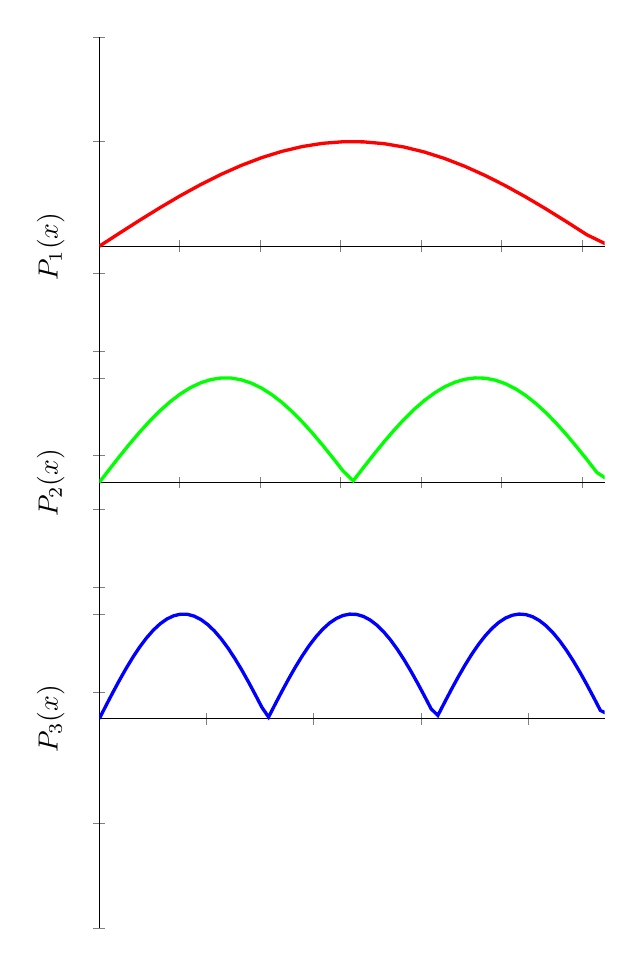
\begin{tikzpicture}
    \begin{axis}
        [
        axis lines=middle,
        axis line style={-},
        ymin=-1, ymax=1,
        xmin=0, xmax = pi,
        ylabel={$P_1(x)$},
        ytick={-1,-0.5,...,0.5,1},
        yticklabels={,,},
        xticklabels={,,},
        ylabel near ticks,
        ]
        \addplot[red, very thick,samples=200,domain=0:8*pi] {abs((sin(deg(x+pi))/2)*-1)};
    \end{axis}
    \begin{axis}
        [
        yshift=-3cm,
        axis lines=middle,
        axis line style={-},
        ymin=-1, ymax=1,
        xmin=0, xmax = 2*pi,
        ylabel={$P_2(x)$},
        ytick={-1,-0.5,...,0.5,1},
        yticklabels={,,},
        xticklabels={,,},
        ylabel near ticks,
        ]
        \addplot[green, very thick,samples=200,domain=0:8*pi] {abs((sin(deg(x+pi))/2)*-1)};
    \end{axis}
    \begin{axis}
        [
        yshift=-6cm,
        axis lines=middle,
        axis line style={-},
        ymin=-1, ymax=1,
        xmin=0, xmax = 3*pi,
        ylabel={$P_3(x)$},
        ytick={-1,-0.5,...,0.5,1},
        yticklabels={,,},
        xticklabels={,,},
        ylabel near ticks,
        ]
        \addplot[blue, very thick,samples=200,domain=0:8*pi] {abs((sin(deg(x+pi))/2)*-1)};
    \end{axis}
\end{tikzpicture}
